%% ceci est un commentaire 
%% il faut toujours commencer par \documentclass[type de papier, taille de texte]{sytle du document}
\documentclass[a4paper,10pt]{report} %%%% sytle du document : report/book/article


%%%%%%%%%%%%%%%%%%%%%%%%%%%%%%%%%%%%%%%%%%%%%%%%%%%%%%%%%%%%%%%%%%%%%%%%%%%%%%%
%% la suite est une collection des "package" ou des "librararies" pour utiliser des codes spécifiques
%% il vous suffit de les copie-coller quand vous créez un nouveau document TeX (ou bien en ajouter plus si besoin).
\usepackage[utf8]{inputenc} %% pour les accents en français
\usepackage[frenchb]{babel} %% pour un format français
\usepackage{graphicx} %% pour afficher des graphiques
\usepackage{amsmath} %% pour écrire des symboles (maths), des équations, etc.
\usepackage{amssymb}
\usepackage{xcolor}
\usepackage{bm} %% pour lister des citations/la biblio
\usepackage{hyperref} %% pour inserer des liens internet
\usepackage{cleveref} %% pour faire des références uax équations, tableaux, etc.
%\usepackage{ulem}
%\usepackage{setspace} %% pour changer l'espace entre les lignes
%\linespread{1.6} %% pour changer l'espace entre les lignes

%%%%%%%%%%%%%%%%%%%%%%%%%%%%%%%%%%%%%%%%%%%%%%%%%%%%%%%%%%%%%%%%%%%%%%%%%%%%%%%
\title{\textbf{Equation des ondes en 2D}} %% choissez un titre approprié à votre sujet
\author{par\\ZHANG Xunjie\\pour le UE Méthodes numériques pour les EDP Mécanique M1 } %% utilisez \\ pour une novuelle ligne
\date{fait le 31 mai 2017} %% pour afficher la date actuelle commenter cette ligne

%%%%%%%%%%%%%%%%%%%%%%%%%%%%%%%%%%%%%%%%%%%%%%%%%%%%%%%%%%%%%%%%%%%%%%%%%%%%%%%
%% TOUT ce qui va dans votre rapport doit être entre \begin{document} & \end{document}
\begin{document}
\selectlanguage{french} %% format français
\maketitle %% pour afficher le titre
\tableofcontents %% pour afficher/compiler le sommaire automatiquement
\listoffigures %% pour lister les figures
%%%%%%%%%%%%%%%%%%%%%%%%%%
%%%%%%%%%%%%%%%%%%%%%%%%%%%%%%%%%%%%%%%%%%%%%%%%%%%%%%%%%%%%%%%%%%%%%%%%%%%%%%%
\chapter{Introduction} 
\section{Problème physique}
On considère des oscillations à la surface d'un liquide contenu dans un generateur des ondes . La surface libre du liquide est à $z=h(x,y,t)$, et paroi à $z=0$ ; la frontière du réseroir est de forme carré , i.e. , à $x=\pm L$,$-L\leq y\leq L$et$y=\pm L$,$-L\leq x\leq L$ .On néglige les effects de viscosité et on suppose que le fluide est un liquide incompressible . 
\begin{figure}[h]
\centering
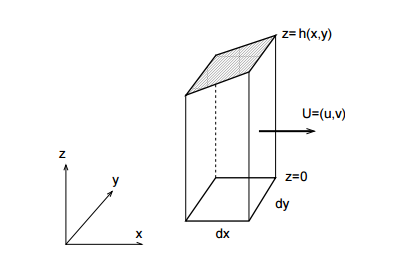
\includegraphics[width=0.8\textwidth]{fig/figure1.png}
\caption{Problem physique d'etude}
\end{figure}

On considère la perturbation de la surface libre $\xi(x,y,t)$ :$=h(x,y,t)-h_0$ soit faible , donc on obtient l'équation de propagation :
\begin{equation}
\frac{\partial ^2\xi}{\partial t^2}=c_0^2\Big(\frac{\partial ^2\xi}{\partial x^2}+\frac{\partial ^2\xi}{\partial y^2}\Big)
\end{equation}
où $c_0$ est la célerité des ondes de surface . Les conditions initiales correspondent à la perturbation et vitesse 

\begin{equation}
\xi(x,y,t=0)=0\,\,\,\,\,\,\,\frac{\partial \xi}{\partial t}(x,t,t=0)=0
\end{equation}

\section{Modifisations des conditions limites}
Bilan de masse pour le cylindre de volume $hdxhy$ s'ecrit:
\begin{equation}
\frac{\partial}{\partial t}(\rho h)+\frac{\partial \rho h u}{\partial x}+\frac{\partial \rho h v}{\partial y}=0
\end{equation}

Pour obtenir  une condition sur $\xi$ , on utilise la combinaison suivant $\vec{n}$
 Sauf à $x=L$ , la vitesse normale est $u\cdot n=\frac{Ag}{\omega}\sin(\omega t)$ 

Bilan de quandité de mouvement s'écrit :
\begin{equation}
\frac{\partial \rho h u}{\partial t}+\frac{\partial \rho h u^2}{\partial x}+\frac{\partial \rho h uv}{\partial y}+\frac{\partial p}{\partial x}=0
\end{equation}
\begin{equation}
\frac{\partial \rho h v}{\partial t}+\frac{\partial \rho h uv}{\partial x}+\frac{\partial \rho h v^2}{\partial y}+\frac{\partial p}{\partial y}=0
\end{equation}

On considère que le fluide est un liquide incompressible , et que la perturbation de la surface libre  $\xi=h-h_0$ est faible .

On peut alors considèrerque la répartition de pression reste hydrostatique :
\begin{equation}
p(x,y,z,t)=p_0+\rho g(h-z)
\end{equation}

On note que : $h=h_0=\xi$,$p=p_s+\rho g\xi$ , les équations vient :
$$\frac{\partial \xi}{t}=h_0 \frac{\partial u}{\partial x}+h_0 \frac{\partial v}{\partial y}=0$$
$$\frac{\partial u}{\partial t}=g\frac{\partial \xi}{\partial x}$$
$$\frac{\partial v}{\partial t}=g\frac{\partial \xi}{\partial y}$$

Après dérivations des trois équations , on obtient :
\begin{equation}
\frac{\partial ^2\xi}{\partial t^2}-gh_0\Big(\frac{\partial ^2\xi}{\partial x^2}+\frac{\partial ^2\xi}{\partial y^2}\Big)=0
\label{propagation}
\end{equation}
\begin{equation}
\frac{\partial\vec{U}\cdot\vec{n}}{\partial t}+g\frac{\partial \xi}{\partial n}=0
\label{conditionlimite}
\end{equation}

Donc , dans l'equation \ref{propagation}, on trouve
 $$c_0=\sqrt{gh_0}$$

On déduit la condition aux limites sur $\xi$ dans l'équation \ref{conditionlimite}
\begin{equation}
\frac{\partial \xi}{\partial n}=-\frac{1}{g}\frac{\partial\vec{U}\cdot\vec{n}}{\partial t}
\end{equation}

Donc pour les frontières $x=L$ et $y=\pm L$:
$$\frac{\partial \xi}{\partial x}\Big|_{x=L}=0$$
$$\frac{\partial \xi}{\partial y}\Big|_{y\pm L}=0$$

PPour la frontière $x=-L$:
$$\frac{\partial \xi}{\partial x}\Big|_{x=-L}=-\frac{1}{g}\frac{\partial\vec{U}\cdot\vec{n}}{\partial t}=-A\cos(\omega t)$$

%%%%%%%%%%%%%%%%%%%%%%%%%%%%%%%%%%%%%%%%%%%%%
%%%%%%%%%%%%%%%%%%%%%%%%%%%%%%%%%%%%%%%
\chapter{Solution analytique } 
\section{Solution analytique en \textbf{1D}}
Pour 1D , on a l'équation de propagation :
\begin{equation}
\frac{\partial ^2\xi}{\partial t^2}=c_0^2\frac{\partial ^2\xi}{\partial x^2}
\label{1d}
\end{equation}

Dans l'équation \ref{1d} , On replace $\xi$ par la forme $\xi=B\sin(k(x-x_0)-\omega t)\,\,\,,t<\frac{2L}{c_0}$ besion de montrer,\\

 à gauche :
$$\frac{\partial \xi}{\partial t}=-\omega B\cos(k(x-x_0))-\omega t)$$
$$\frac{\partial^2 \xi}{\partial t^2}=-\omega^2B\sin(k(x-x_0))-\omega t)$$

à droite :
$$\frac{\partial \xi}{\partial x}=k B\cos(k(x-x_0))-\omega t)$$
$$\frac{\partial^2 \xi}{\partial x^2}=-k^2B\sin(k(x-x_0))-\omega t)$$

Droite=gauche ,on trouve :
$$k=\frac{\omega}{c_0}$$

Avec la condition limite $\frac{\partial \xi}{\partial x}\Big|_{x=-L}=-A\cos(\omega t)$, on trouve :
$$B=-\frac{A}{k}=-\frac{Ac_0}{\omega}$$

\section{Solution pour t $\geq\frac{2L}{c_0}$}
L'onde arrive la frontière $x=L$ à l'instant $t=\frac{2L}{c_0}$ , après l'onde va propager vers la direction opposite avec la même vitesse opposite , donc , quand $t>\frac{2L}{c_0}$ , il y aura une superposition de deux ondes avec même $\omega$ .

%%%%%%%%%%%%%%%%%%%%%%%%%%%%%%%%%%%%%%%%%%%%%
%%%%%%%%%%%%%%%%%%%%%%%%%%%
\chapter{Méthodes numérique} 
\section{Stabilité}

\begin{equation}\frac{h^{n+1}_{i,j}-2h^{n}_{i,j}+h^{n-1}_{i,j}}{\Delta t^{2}}=C^{2}_{0}\frac{h^{n}_{i+1,j}-2h^{n}_{i,j}+h^{n}_{i-1,j}}{\Delta x^{2}}+C^{2}_{0}\frac{h^{n}_{i,j+1}-2h^{n}_{i,j}+h^{n}_{i,j-1}}{\Delta y^{2}}
\end{equation}

\begin{equation}h^{n+1}_{i,j}-2h^{n}_{i,j}+h^{n-1}_{i,j}=\frac{C^{2}_{0}\Delta t^{2}}{\Delta x^{2}}(h^{n}_{i+1,j}-2h^{n}_{i,j}+h^{n}_{i-1,j})+\frac{C^{2}_{0}\Delta t^{2}}{\Delta x^{2}}(h^{n}_{i,j+1}-2h^{n}_{i,j}+h^{n}_{i,j-1})
\end{equation}

On pose: $$C_{FL1}=\frac{C_{0}\Delta t}{\Delta x}$$ et$$C_{FL12}=\frac{C_{0}\Delta t}{\Delta y}$$

On introduit la perturbation : $$\varepsilon^{n}_{i,j}=\psi^{n}e^{I\omega_{1}i\Delta x}e^{I\omega_{2}j\Delta y}$$

Donc: \begin{equation}\psi^{n+1}-\psi^{n}+\psi^{n-1}=C_{FL1}^{2}(\psi^{n}e^{I\omega_{1}i\Delta x}-2\psi^{n}+\psi^{n}e^{-I\omega_{1}i\Delta x}+C_{FL2}^{2}(\psi^{n}e^{I\omega_{2}i\Delta y}-2\psi^{n}+\psi^{n}e^{-I\omega_{2}i\Delta y})
\end{equation}

Or $G=\frac{\psi^{n+1}}{\psi^{n}}=\frac{\psi{n}}{\psi^{n-1}}$, on a alors:

$$G-2+\frac{1}{G}=2C_{FL1}^{2}(\cos(\omega_{1}\Delta x)-1)+2C_{FL2}^{2}(\cos(\omega_{2}\Delta y)-1)$$

$$G-2+\frac{1}{G}=-4C_{FL1}^{2}(\sin^{2}(\frac{\omega_{1}\Delta x)}{2})-4C_{FL2}^{2}(\sin^{2}(\frac{\omega_{2}\Delta y)}{2})$$
On pose: $y_{1}=sin(\frac{\omega_{1}\Delta x}{2})$, $y_{2}=sin(\frac{\omega_{2}\Delta y}{2})$

\begin{equation}
G^{2}+(4C_{FL1}^{2}y_{1}^{2}+4C_{FL2}^{2}y_{2}^{2}-2)G+1=0
\end{equation}

\begin{equation}
G^{2}+2\alpha G+1=0
\end{equation}
Avec $$\alpha=2C_{FL1}^{2}y_{1}^{2}+2C_{FL2}^{2}y_{2}^{2}-1$$

Pour étudier la stabilité, il faut $\big|G\big|\leq 1$.

si $\Delta > 0$:
$$G_{1,2}=\frac{-2\alpha\pm\sqrt{4\alpha^{2}-4}}{2}=-\alpha\pm\sqrt{\alpha^{2}-1}$$
$$G_{1}*G_{2}=1$$ 
$$\Longrightarrow\big|G_{1}\big|\geq1\,\,\,\,ou\,\,\,\,\big|G_{2}\big|\geq1$$. Donc, il est instable.

si $\Delta \leq 0$:
$$\Delta=4\alpha^{2}-4\leq0$$
$$\alpha^{2}\leq1$$
$$1\leq \alpha\leq1$$ On peut trouver que $C_{FL1}^{2}+C_{FL2}^{2}\leq 1 $
$$ C_{FL1}^{2}+C_{FL2}^{2}=\frac{C_{0}^{2}\Delta t^{2}}{h^{2}}=C_{FL}^{2}\leq 1$$ 
Alors:
$$C_{FL}\leq1$$

%Dand notre cas, le pas de discrétisation sont égaux dx=dy car Nx=Ny, donc $h=\frac{dx}{\sqrt{2}}$.
%La condition de stabilité est donc :
%$$\frac{C_{0}dt}{h}=\frac{C_{0}dt*\sqrt{2}}{dx}\leq1$$
%\begin{equation}
%\frac{C_{0}dt}{dx}\leq\frac{1}{\sqrt{2}}=0.7
%\end{equation}


\section{Consistance}

\begin{equation}\frac{h^{n+1}_{i,j}-2h^{n}_{i,j}+h^{n-1}_{i,j}}{\Delta t^{2}}=C^{2}_{0}\frac{h^{n}_{i+1,j}-2h^{n}_{i,j}+h^{n}_{i-1,j}}{\Delta x^{2}}+C^{2}_{0}\frac{h^{n}_{i,j+1}-2h^{n}_{i,j}+h^{n}_{i,j-1}}{\Delta y^{2}}
\label{1}
\end{equation}

\begin{equation}
h^{n\pm1}_{i,j}=h^{n}_{i,j}\pm dt\frac{\partial h}{\partial t}+\frac{dt^{2}}{2}\frac{\partial^{2}h}{\partial t^{2}}\pm \frac{dt^{3}}{6}\frac{\partial^{3}h}{\partial t^{3}}+\frac{dt^{4}}{24}\frac{\partial^{4}h}{\partial t^{4}}\pm\bigcirc(dt^{5})
\end{equation}


\begin{equation}
h^{n}_{i\pm1,j}=h^{n}_{i,j}\pm dx\frac{\partial h}{\partial x}+\frac{dx^{2}}{2}\frac{\partial^{2}h}{\partial x^{2}}\pm \frac{dx^{3}}{6}\frac{\partial^{3}h}{\partial x^{3}}+\frac{dx^{4}}{24}\frac{\partial^{4}h}{\partial x^{4}}\pm\bigcirc(dx^{5})
\end{equation}


\begin{equation}
h^{n}_{i,j\pm1}=h^{n}_{i,j}\pm dy\frac{\partial h}{\partial y}+\frac{dy^{2}}{2}\frac{\partial^{2}h}{\partial y^{2}}\pm \frac{dy^{3}}{6}\frac{\partial^{3}h}{\partial y^{3}}+\frac{dy^{4}}{24}\frac{\partial^{4}h}{\partial y^{4}}\pm\bigcirc(dy^{5})
\end{equation}

On peut remplacer l'équation \ref{1} par les équations avants. Donc il est:
$$\frac{\partial^{2}h}{\partial t^{2}}+\frac{dt^{2}}{12}\frac{\partial^{4}h}{\partial t^{4}}+\bigcirc(dt^{4})=C^{2}_{0}(\frac{\partial^{2}h}{\partial x^{2}}+\frac{dx^{2}}{12}\frac{\partial^{4}h}{\partial x^{4}})+\bigcirc(dx^{4})+C^{2}_{0}(\frac{\partial^{2}h}{\partial y^{2}}+\frac{dy^{2}}{12}\frac{\partial^{4}h}{\partial y^{4}})+\bigcirc(dy^{4})$$

On obtient donc l'erreur troncature:

\begin{equation}
ErrT=\frac{dt^{2}}{12}\frac{\partial^{4}h}{\partial t^{4}}-C^{2}_{0}\frac{dx^{2}}{12}\frac{\partial^{4}h}{\partial x^{4}}-C^{2}_{0}\frac{dy^{2}}{12}\frac{\partial^{4}h}{\partial y^{4}}+\bigcirc(dt^{4},dx^{4},dy^{4})
\label{2}
\end{equation}

Ce schéma est consistant.Il est conditionnellement stable et consistant.

\section{Dispersion}
On a :
$$\frac
{\partial^{4}h}{\partial t^{4}}=C_{0}^{2}\frac{\partial^{2}}{\partial t ^{2}}(\frac{\partial^{2}h}{\partial x^{2}}+\frac{\partial^{2}h}{\partial y^{2}})=C_{0}^{2}\frac{\partial^{2}}{\partial x ^{2}}(\frac{\partial^{2}h}{\partial t^{2}})+C_{0}^{2}\frac{\partial^{2}}{\partial y ^{2}}(\frac{\partial^{2}h}{\partial t^{2}})$$$$=C_{0}^{4}(\frac{\partial^{4}h}{\partial x^{4}}+\frac{\partial^{4}h}{\partial x^{2}\partial y^{2}})+C_{0}^{4}(\frac{\partial^{4}h}{\partial y^{4}}+\frac{\partial^{4}h}{\partial x^{2}\partial y^{2}})
$$

En remplaçant le $\frac
{\partial^{4}h}{\partial t^{4}}$ dans l'équation \ref{2}, on obtient:
$$ErrT=\frac{C_0^2dx^2}{12}(C_{FL}^2-1)*\frac{\partial^{4}h}{\partial x^{4}}+\frac{C_0^2dy^2}{12}(C_{FL}^2-1)*\frac{\partial^{4}h}{\partial y^{4}}+\frac{dt^2C_0^4}{6}\frac{\partial^{4}h}{\partial x^{2}\partial y^{2}}+\bigcirc(dt^{2},dx^{2},dy^{2})$$
On peut dire que l'erreur de troncature est principalement de la dispersion numérique.



\section{Conditions initials sous Matlab}
\begin{figure}[h]
\centering
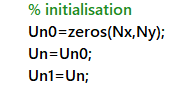
\includegraphics[width=0.72\textwidth]{fig/figure4.png}
\caption{Conditions initials}
\label{initial}
\end{figure}

Dans la figure \ref{initial} , $Un0=zeros(Nx,Ny)$,$Un=Un0$ est bien correspondant à condition initial $\xi(x,y,t=0)=0$ . Et $Un1=Un$ est satisfait à la condition initail $\frac{\partial \xi}{\partial t}(x,y,t=0)=0$
\section{Programmer Matlab}
Sur moodle , vous pouvez trouver les codes Matlab .
%%%%%%%%%%%%%%%%%%%%%%%%%%%%%%%%%%%%%%%%%%%%%%%%%%%%%%%%%%%%%%%%%%%%%
\chapter{Etude numérique}
\section{Cas test}

Au début on s'interes à t = 1s :
\begin{figure}[h]
\centering
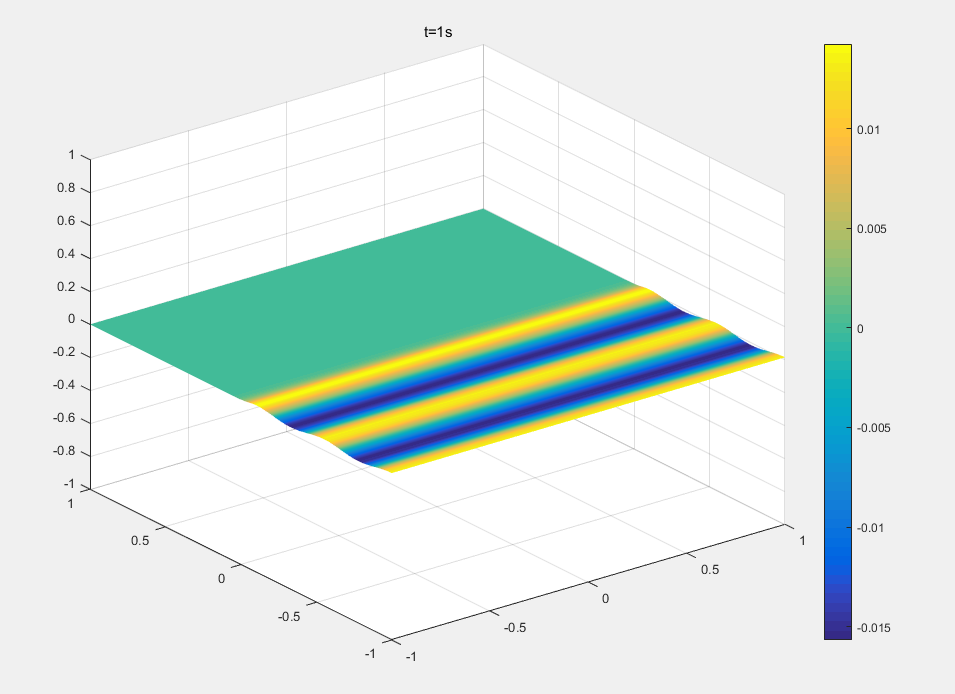
\includegraphics[width=0.9\textwidth]{fig/figure5.png}
\caption{A t=1s , snapshot de la surface libre}
\label{5}
\end{figure}

C'est la snapshot à l'instante t=1s . Dans le \ref{5} on voir il y a pas de vibration , parce-que l'onde ne propage pas cette zone . donc il est une plant initiale . Le point intéressé (0,0) commence vibration après cette l'instante .\\\\\\\\\\\\\\\ 
\begin{figure}[h]
\centering
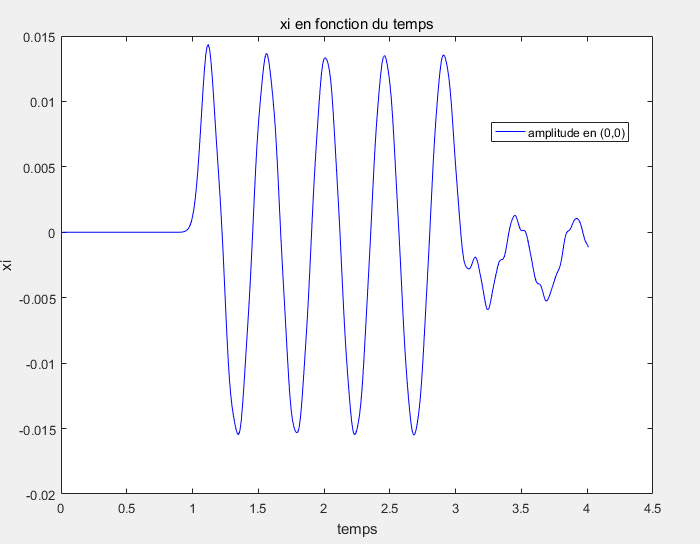
\includegraphics[width=0.7\textwidth]{fig/figure10.png}
\caption{La fonction de $\xi(0,0,t)$ en fonction du temps}
\label{10}
\end{figure}

 Dans la figure \ref{10} , on remarque qu'avant l'instante t=1s , il n'y a pas de vibration , c'est bien satisfait la figure \ref{5} . A l'instante t=3s , l'onde revient à la position (0,0) , donc il aura une superposition , donc l'amplitude ou $\xi$ va changer . Pour moi , $\omega=14.0$ , c'est une superposition diminuée.  
\section{Precision spatial}
\begin{figure}[h]
\centering
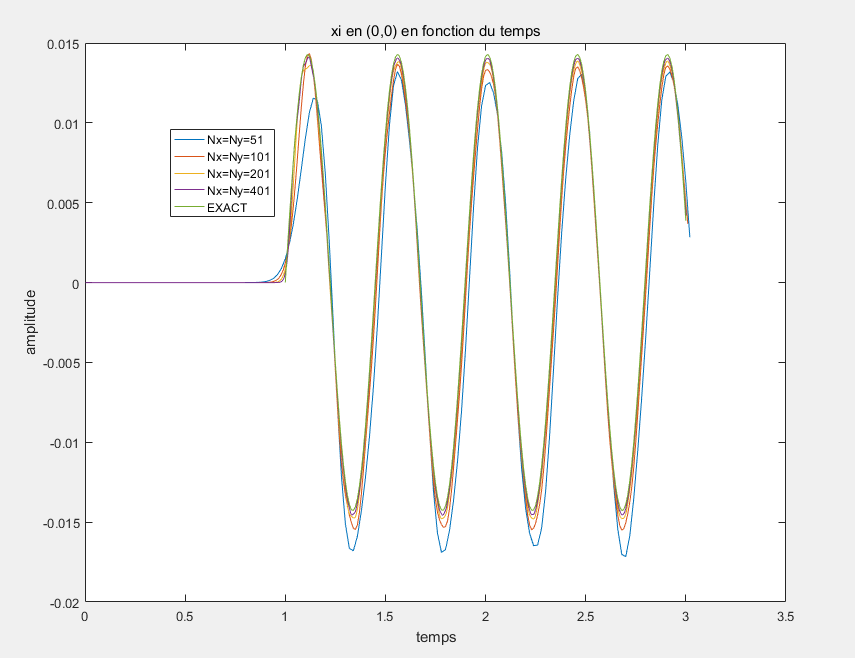
\includegraphics[width=0.7\textwidth]{fig/figure8.png}
\caption{La fonction de $\xi(0,0,t)$ en fonction du temps pour tous les Nx}
\label{8}
\end{figure}

Dans la figure \ref{8} , on trace les fonctions de $\xi(0,0,t)$ pour tous les Nx ,ansique la solution exact . On trace les fonctions jusqu'à t=3s , parce-que d'après t=3s , il y a une superposition . A cause de sans vibration avant t=1s pour la solution exact de point (0,0) , on utilise deux façons pour pragrammer . Une façon , c'est fonction heaviside , une autre est changer t par t-1. , çava va dire que la solution va transpose à droite en 1 second . 

\begin{figure}[h]
\centering
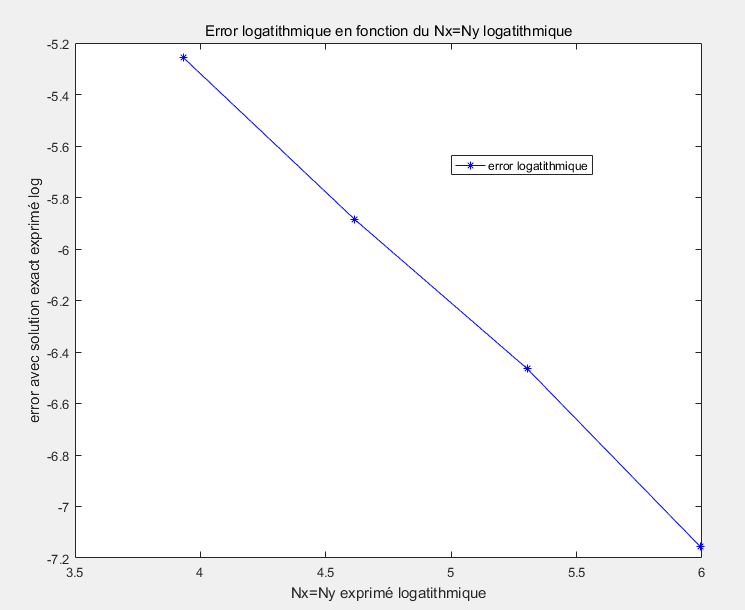
\includegraphics[width=0.75\textwidth]{fig/figure7.png}
\caption{Error en fonction du Nx logatithmique}
\end{figure}.\\\\\\\\
Dans le figure \ref{9} on trace error en fonction du Nx logatithmique . L'error est l'différence absolute maximale  entre solution simulation et solution exact sur le point (0,0) pendant 3 seconds .
\begin{figure}[h]
\centering
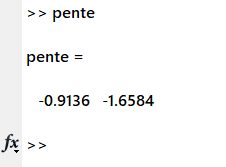
\includegraphics[width=0.54\textwidth]{fig/figure9.png}
\caption{pente}
\label{9}
\end{figure}

Dans la figure \ref{9} , Nx=[51,101,201,401] .Sous matlab , on trouve la pente est prêsque -1 , il est bien satifait théorique analytique en calculant l'error troncature  .




\section{Précision temporelle}
\begin{figure}[h]
\centering
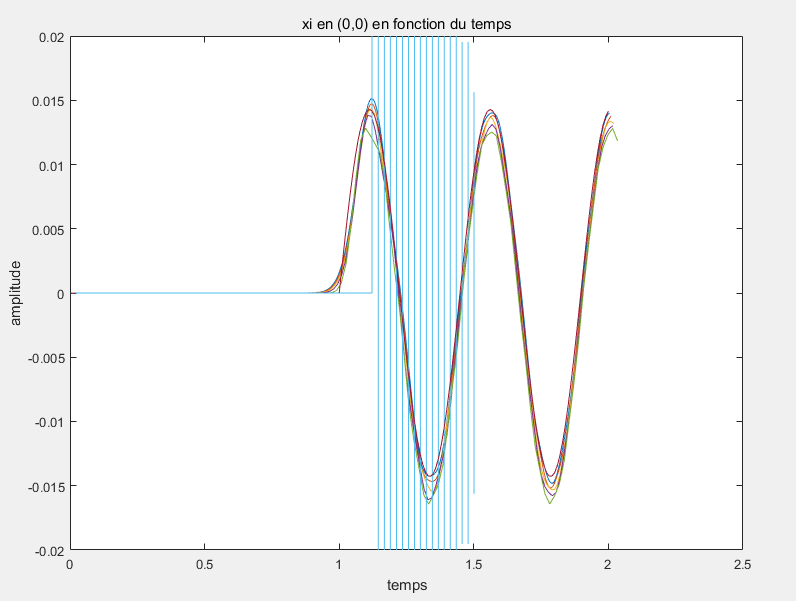
\includegraphics[width=0.7\textwidth]{fig/figure12.png}
\caption{La fonction de $\xi(0,0,t)$ en fonction du CFL logatithmique}
\label{12}
\end{figure}

Dans la figure \ref{12} , on trace les fonction des CFL , CFL=[0.1,0.3,0.5,0.7,0.9,1.1], la ligne blue est sous la fonction CFL=1.1 , il diverge avec les solutions simulations d'autres .

\begin{figure}[h]
\centering
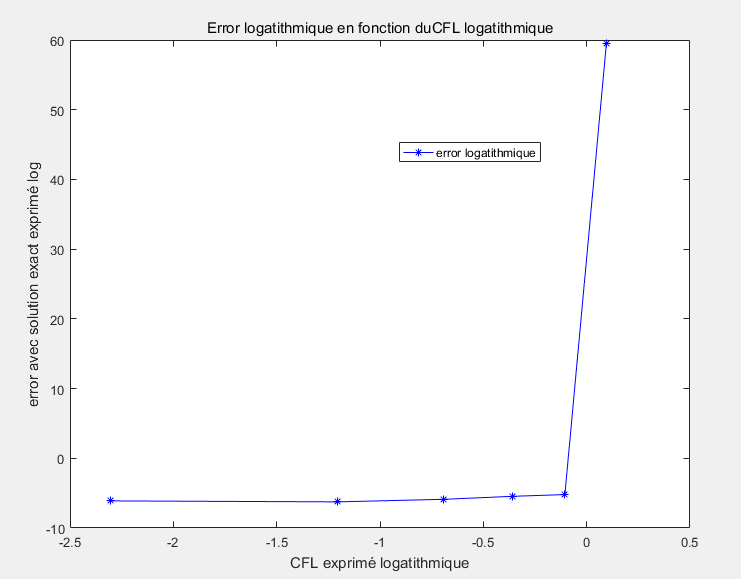
\includegraphics[width=0.7\textwidth]{fig/figure11.png}
\caption{L'error en fonction du CFL logatithmique}
\label{11}
\end{figure}

Dans la figure \ref{11} , l'error logatithmique est convergente quand CFL sont [0.1,0.3,0.5,0.7,0.9] , d'autre part , quand CFL est supérieur que 1 , l'error est plus grande qu'avant , c'est bien satisfait que CFL$\leq 1$ .

\begin{figure}[h]
\centering
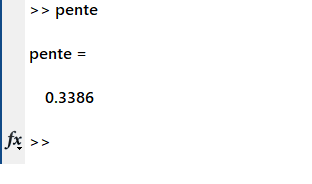
\includegraphics[width=0.7\textwidth]{fig/figure13.png}
\caption{pente}
\label{13}
\end{figure}

Dans la figure \ref{13} , sous matlab , on trouve la pent est 0.34 pour l'error logatithmique en fonction CFL logatithmique . Dans l'analythique théorie , quand CFL augmente , dt augemente , error augement , donc la pente est positive .  

\section{Nouvelle conditions à $x=-L$}
\begin{figure}[h]
\centering
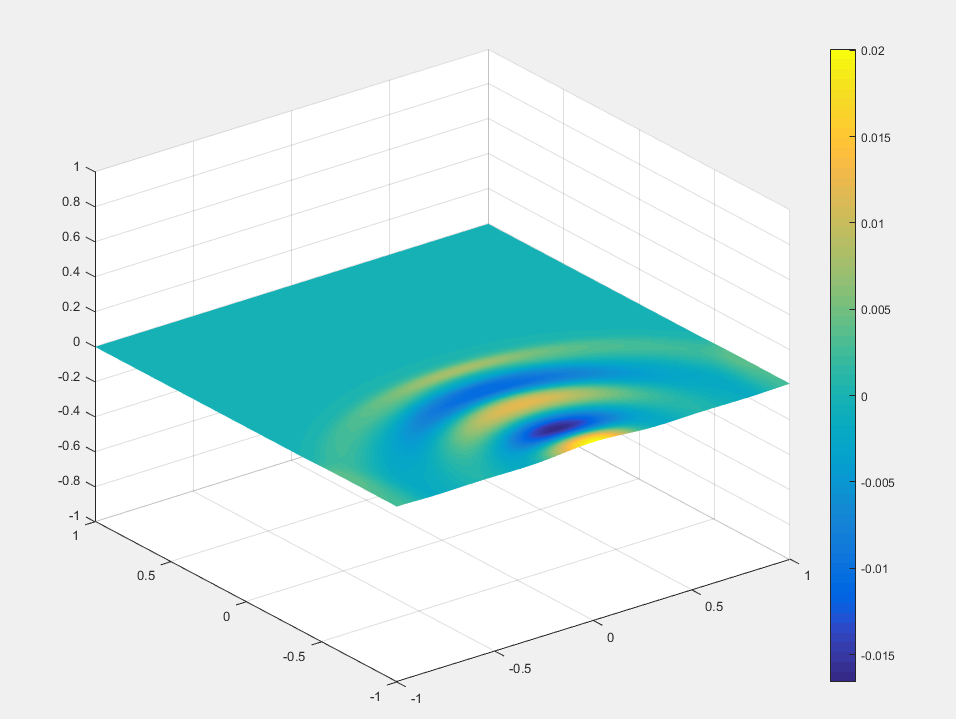
\includegraphics[width=0.7\textwidth]{fig/figure2.png}
\caption{A t=1s , snapshot de la surface libre}
\label{2}
\end{figure}
Dans la figure \ref{2} , on trace la snapshot à t=1s , pour cette nouvelle contidions limtes on ajoute $\frac{\partial \xi}{\partial y}\Big|_{-L,\frac{L}{10}<|y|<L}=0$ .Et on pour $|y|<\frac{L}{10}$ , on utilise la même qu'en avant .
On remarque l'on va propager vers autour de l'entrée .\\\\\\\\

\begin{figure}[h]
\centering
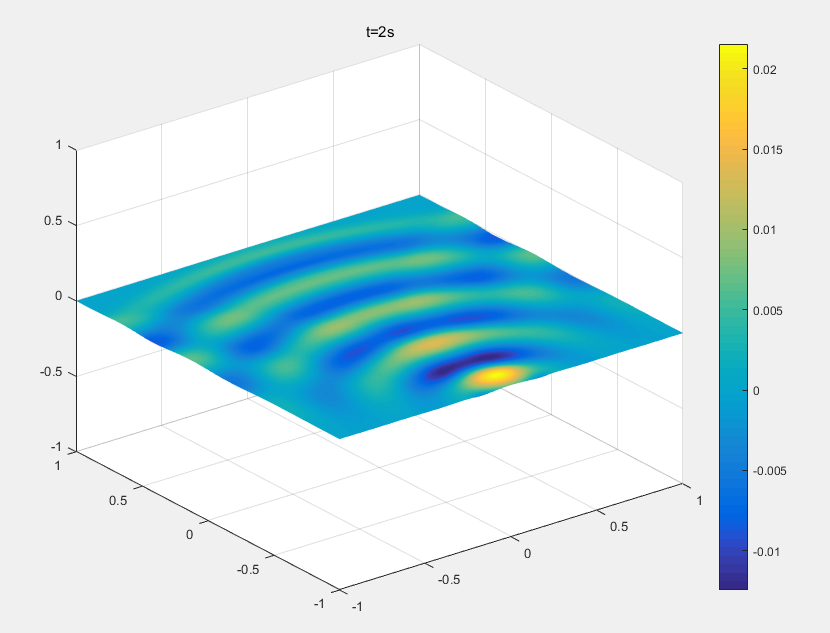
\includegraphics[width=0.9\textwidth]{fig/figure3.png}
\caption{A t=2s , snapshot de la surface libre}
\end{figure}
\label{sss3}

Dans la figure 4.10 , on trace la snapshot à l'instant t=2s , et on peut voir les arcs  évidament , on dit que si on a un'entrée ponctuel au milieu , on peut voir les cercles autour de la centre .
\chapter{Conclusion} 
Dans cette séance de TP , on a fait une bonne etude d'équation des ondes en 2D .Au début , on modifie les conditions limites de Neumann à partie l'quation de masse et quantité de mouvement , ensuite on cherche la solution exact . ensuite on utilise matlab pour faire les simulations  . On programmer les codes et on trouver les résultats . \\\\
On etude la stabilité et consistance ,  on retrouve dans le code , l'erreur spatial diminue quand Nx augement .Pour l'erreur temporelle , on lasse Nx constante , on introduit une serie de CFL , on on dit quand CFL est inférieur ou égale que 1 , la solution similation converge la solution numérique .\\\\



\end{document}
\grid
